\documentclass[12pt,titlepage]{article}
\usepackage{mathtools}
\usepackage[italian]{babel}
\usepackage{graphicx}
\usepackage[utf8]{inputenc}
\usepackage{float}
\usepackage{tabularx}
\usepackage{chngpage}
\usepackage[toc,page]{appendix}
\usepackage{gensymb}
\usepackage{subcaption}

\addtolength{\topmargin}{-.875in}
\textheight=674pt

\title{\textbf{EQUAZIONE DI STATO DEI GAS} }
\author{Canteri Marco\\Mura Francesca}
\date{Maggio 2015}

\begin{document}
	\maketitle
	\tableofcontents
	\renewcommand{\abstractname}{Abstract}
	
	\begin{abstract}
In questa esperienza andremo a misurare la pressione di una data quantità di gas (aria), a volume $V$ costante, al variare della temperatura $T$.
Andremo a variare la temperatura tra un valore minimo di circa $0^{\degree}$ C ad un valore massimo di circa $20^{\degree}$ C.
In seguito stimeremo la temperatura dello zero assoluto a partire dai dati raccolti.
	\end{abstract}
	
\newpage
\section{Obiettivi}
\begin{itemize}
\item Misurazione della pressione di un gas con un manometro d'acqua
\item Uso del barometro per la misurazione della pressione atmosferica
\item Studio della relazione tra pressione e temperatura per un gas a volume costante
\item Introduzione all'uso del termometro a gas
\end{itemize}

\section{Materiali e strumenti}
\begin{itemize}
\item 1 contenitore, capacità di circa 3 litri
\item 1 recipiente cilindrico di vetro (bottiglia con due rubinetti, capacità 0.6 litri)
\item 1 termometro digitale con risoluzione di lettura $0.01^{\degree}$ C
\item 1 agitatore magnetico
\item 1 manomentro ad acqua con relativa supporteria
\item 1 barometro per la misura della pressione atmosferica (in comune a tutti i gruppi)
\item 1 siringa di plastica
\end{itemize}

\newpage
\section{Introduzione}
\subsection{Preparazione dell'apparato sperimentale}

Per questa esperienza è d'obbligo prestare una particolare attenzione alla costruzione dell'apparato sperimentale, in quanto anche piccole dimenticanze o imprecisioni possono causare variazioni notevoli nelle misurazioni.
Si proceda quindi con la preparazione dell'apparato: versare un pò d'acqua nel contenitore, posarlo sopra l'agitatore magnetico ed inserire l'ancoretta magnetica al suo interno; controllare quindi che l'agitatore magnetico faccia vibrare l'ancoretta che, a sua volta, deve garantire la rotazione dell'acqua che la circonda.
Questa prima verifica è necessaria in quanto l'acqua diventerà il bagno termico per tutta la durata dell'esperimento e quindi il mescolamento dell'agitatore termico è una condizione necessaria per l'omogeneità dell'acqua che andrebbe, in sua assenza, a stratificarsi in base alla sua temperatura.
Controllare quindi che l'interno della bottiglia contenente il gas non sia in nessun modo bagnato e, tenendo aperti i rubinetti, fissarla stabilmente aòò'apposito sostegno in modo che essa possa restitere alla spinta idrostatica ed in modo da permettere il funzionamento dell'agitatore magnetico.
Collegare quindi un ramo del manometro ad uno dei rubinetti della bottiglia ed, aiutandosi con la siringa di plastica, versare acqua nel manometro tenendo i due rubinetti alla stessa altezza e prestando particolare attenzione in modo da evitare la formazione di bolle d'aria.
Riempire il manometro di acqua il più possibile, prestando attenzione che l'acqua raggiunga il più alto livello possibile non superando la parte rigida trasparente, grazie alla quale saremmo in grado di prendere le misure sulla scala millimetrata posta accanto.
Verificare nuovamente che la bottiglia contenente il gas sia perfettamente asciutta.

\subsection{Termalizzazione iniziale dell'aria}
Procedere quindi con la termalizzazione dell'aria.
Preparare il bagno termico intorno alla bottiglia e tramite il termometro controllare l'uniformità della temperatura, garantita dall'agitatore termico.
Scegliamo di termalizzare inizialmente intorno ai $0^{\degree}$ C per poi salire fino ad una temperatura di circa $20^{\degree}$ C e quindi ridiscendere nuovamente fino al valore iniziale.
Scegliendo questa procedura di misurazione la bottiglia si troverà sempre in sovrapressione rispetto alla pressione atmosferica: in questo caso quindi il manometro dovrà essere montato sul tavolo con il lato libero in grado di salire di circa 80 cm sopra la posizione iniziale (si consiglia quindi di scegliere un valore iniziale che non superi i 20 cm).
Scegliendo di termalizzare il sistema a $0^{\degree}$ C, la presenza di ghiaccio nel bagno dovrà essere presente in maniera predominante rispetto all'acqua: la coesistenza di queste due fasi assicura che la temperatura sia circa uguale allo zero termico.
Immergere quindi la bottiglia nel bagno termico fino al tappo, prestando attenzione che non raggiunga i giunti di connessione dei rubinetti: in questo modo permetteremo una migliore termalizzazione del gas.
Una volta raggiunto l'equilibrio termico alla temperatura iniziale prescelta, aprire il rubinetto e richiuderlo: in questo modo la pressione del gas all'interno della bottiglia viene uniformata con la pressione atmosferica $P_{A}$ ed il volume e le moli del gas rimangono costanti per tutta la durata dell'esperimento.
Procediamo poi con le misurazioni.\\

\subsection{Procedura di misurazione}
Come già affermato, scegliamo di termalizzare inizialmente intorno ai $0^{\degree}$ C per poi salire fino ad una temperatura di circa $20^{\degree}$ C e quindi ridiscendere nuovamente fino al valore iniziale.
Per aumentare la temperatura del bagno di fusione, procediamo sostituendo gradualmente l'acqua del recipiente con acqua più calda; al contrario, per diminuire la temperatura del bagno di fusione, procediamo sostituendo gradualmente l'acqua del recipiente con acqua di fusione.
Ad ogni variazione di temperatura bisogna riportare il valore del volume del gas al valore iniziale, anddando ad alzare o abbassare il ramo libero del manometro.
Andando a incrementare o diminuire la pressione della colonnina d'acqua che preme sul ramo libero del manometro, si va ad incrementare o diminuire la pressione del gas nell'ampolla che permetterà quindi al gas di tornare al suo volume iniziale.
Aspettare un tempo sufficiente per permettere ch eil gas nell'ampolla ed il bagno siano all'equilibrio termico e prendere quindi le misure di temperatura $T$ e di dislivello $\Delta h = h_1 - h_0$, dove $h_0$ è la posizione iniziale e $h_1$ è l'altezza a cui è stato alzato il ramo libero del manometro.
\\
Con questa procedura di misura le incertezze che abbiamo sono esclusivamente di risoluzione e per questo troviamo solamente una incertezza uguale per ogni misura, calcolata come:
\begin{equation}
\sigma (\Delta h) = \sqrt{(\sigma h_1)^2 + (\sigma h_0)^2} = \frac{\Delta X}{\sqrt{6}}
\end{equation}
dove con $\Delta X$ indichiamo il dislivello.
Troviamo quindi una incertezza sulle misurazioni di dislivello pari a $\sigma (\Delta h) = 0.04 m$ .
Per quando riguarda l'incertezza sulle misure di temperatura otteniamo invece una incertezza di risoluzione pari a $\sigma T = 0.1^{\degree}$ C.
Abbiamoscelto quindi di non considerare l'ultima cifra del termometro per varie motivazioni: prima tra tutte quella che questa cifra non era per niente stabile, ma continua ad oscillare tra più valori; la seconda è che questa cifra era relativa alla temperatura di un singolo punto, ovvero il punto in cui il termometro misurava la temperatura del bagno termico, mentre a noi interessava una misura più generale.
Per questo decidiamo di non considerare questa ultima cifra dell'ordine di $0.01^{\degree}$ C relativa alla misura di temperatura in quanto considerata non significativa e poco rilevante per questo esperimento.

\subsection{Pressione assoluta}
Durante tutta la durata dell'esperienza di laboratorio si deve tenere conto di una grandezza, la pressione atmosferica $P_A$, che non è costante nel tempo.
È quindi necessario tenere una traccia oraria relativa alle misurazioni effettuate ed amche prendere numerose misurazione dela pressione atmosferica nell'arco dell'esperienza.
Per effettuare queste misurazioni adoperiamo un barometro.
La pressione $P$ del gas nell'ampolla si ottiene:
\begin{equation}
P = P_A + \rho g h
\end{equation}
dove $P_A$ è la pressione atmosferica calcolata con il barometro, $\rho$ è la densità dell'acqua (pari a $1 \frac{kg}{dm^3}$), $g$
è l'accelerazione di gravità (pari a $9.807 \frac{m}{s^2}$).
L'incertezza su questa misura è data dalla risoluzione del barometro, ovvero $\sigma P = 2 mmHg$.

\section{Analisi dati: primo set}
\subsection{Pressione e temperatura}

\begin{table}[H]
\centering
	\begin{subtable}{.5\textwidth}
		\centering
		\begin{tabular}{|c|c|} \hline
			\textbf{$\Delta h {[cm]}$ } & \textbf{T {[\degree C]} }  \\ \hline
			0 & 0  \\ \hline
			8.5 & 2.3  \\ \hline
			15.9 & 4.1  \\ \hline
			24 & 6.1  \\ \hline
			31.7 & 8.1  \\ \hline
			40.4 & 10  \\ \hline
			49.8 & 12.1  \\ \hline
			56.8 & 14.3  \\ \hline
			63.3 & 16  \\ \hline
			71.8 & 18.4  \\ \hline
			77.6 & 20  \\ \hline
		\end{tabular}
		\caption{Aumento della temperatura}
	\end{subtable}%
	\begin{subtable}{.5\textwidth}
	\centering
	\begin{tabular}{|c|c|} \hline
		\textbf{$\Delta h {[cm]}$ } & \textbf{T {[\degree C]} }  \\ \hline
		77.6 & 20  \\ \hline
		73.4 & 18.8  \\ \hline
		66.2 & 17  \\ \hline
		59.4 & 15  \\ \hline
		52.4 & 13.1  \\ \hline
		44.2 & 11  \\ \hline
		36.2 & 8.9  \\ \hline
		26.5 & 6.9  \\ \hline
		18.9 & 5.1  \\ \hline
		-0.5 & 0  \\ \hline
	\end{tabular}
	\caption{Diminuzione della temperatura}
\end{subtable}

\caption{Dislivello $\Delta h$ in funzione della temperatura $T$}
\end{table}
In Tabella 1.a e Tabella 1.b troviamo riportati i dati raccolti durante la nostra esperienza rispettivamente aumentando e diminuendo la temperatura del bagno termico.
Troviamo graficati tali dati in Figura 1. 

\begin{figure}[H]
\centering
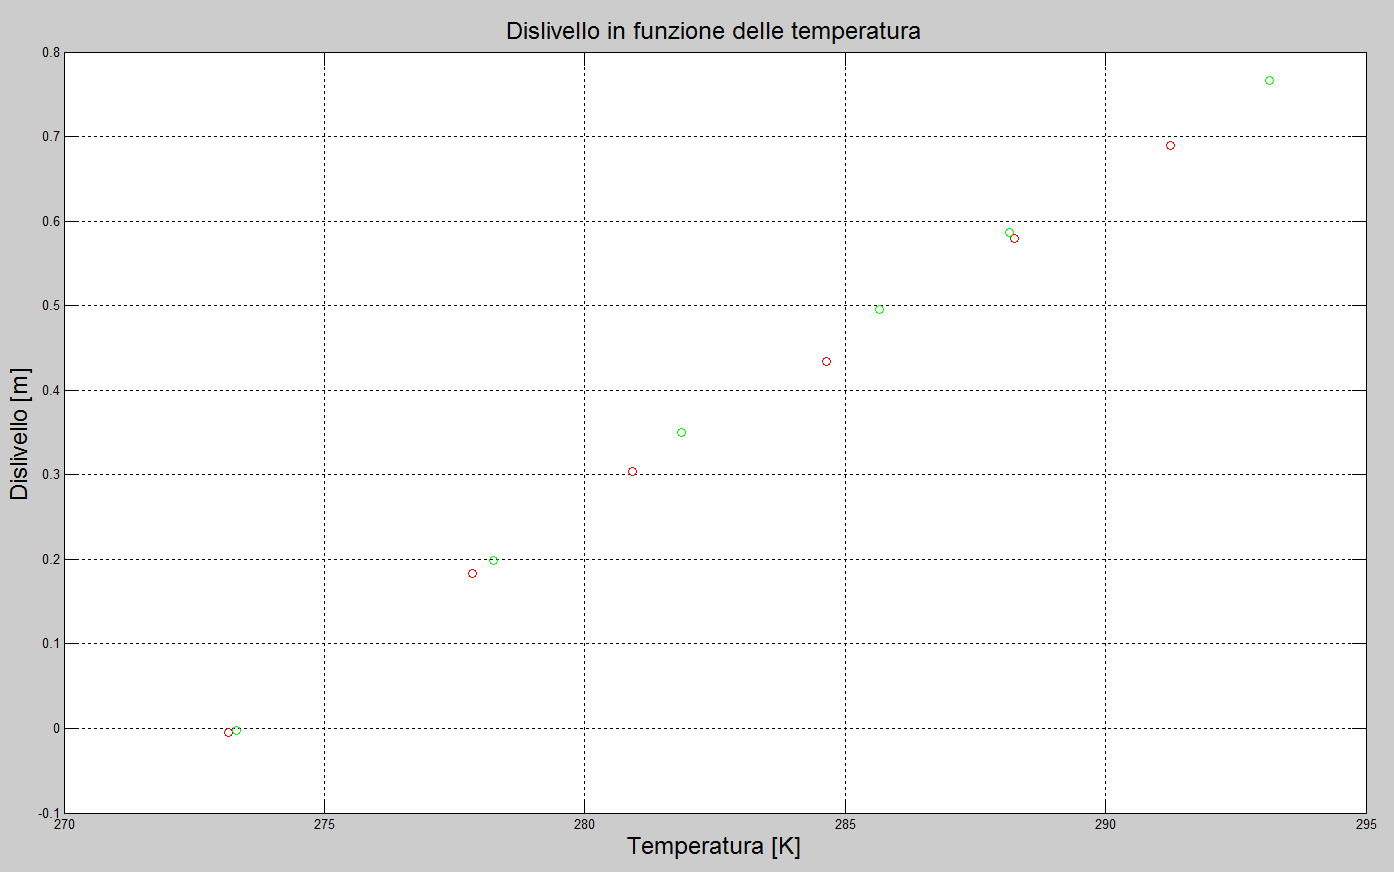
\includegraphics[width=\textwidth]{img/1}
\caption{Grafico di $\Delta h$ in funzione di $T$: in colore rosso i dati riportati in Tabella 1.a ed in colore verde i dati riportati in Tabella 1.b}
\end{figure}

Tramite regressione lineare troviamo la retta $h = A+B\theta$ che meglio interpreta i nostri dati. 
Per farlo dobbiamo innanzitutto trasferire le incertezze dalle ascisse alle ordinate, procediamo quindi a stimare graficamente un valore iniziale della pendenza $b$ della retta e trasferiamo l'incertezza.
\begin{equation}
\sigma(\Delta h)_{tot} = \sqrt{\sigma(\Delta h)^2 + (b\sigma T)^2}
\end{equation}
Le formule per il calcolo sono la \eqref{eq:a} e la \eqref{eq:b} riportate in appendice. Otteniamo:
\[a =-10.7291 \pm 0.0119 \quad  b= 0.0393\pm  0.000041966\]
Verifichiamo la bontà di questo risultato tramite test del $\chi^2$. Ci viene un $\chi^2=948.6366$, decisamente troppo alto come valore.
La retta quindi interpreta malamente i nostri dati. In Figura 1 si può osservare come vari dati non stiano sulla retta. Sempre dal grafico possiamo osservare come i nostri dati possano comportarsi in maniera diversa sopra e sotto i 285 K. Infatti questa è circa la temperatura di rugiada dell'aria. Ci aspettiamo quindi che al di sopra di questa temperatura l'aria si comporti come gas ideale mentre al di sotto ci sarà un contributo dato dal vapore che sarà pari alla tensione di vapor saturo, avremmo quindi una più forte pendenza in funzione della temperatura in quanto la tensione di vapore saturo mostra derivata rispetto alla temperatura maggiore rispetto a quella del gas perfetto.\\
\newline
Dividiamo quindi il problema in due parti divise dalla temperatura di rugiada 285 K.

\begin{figure}[H]
\centering
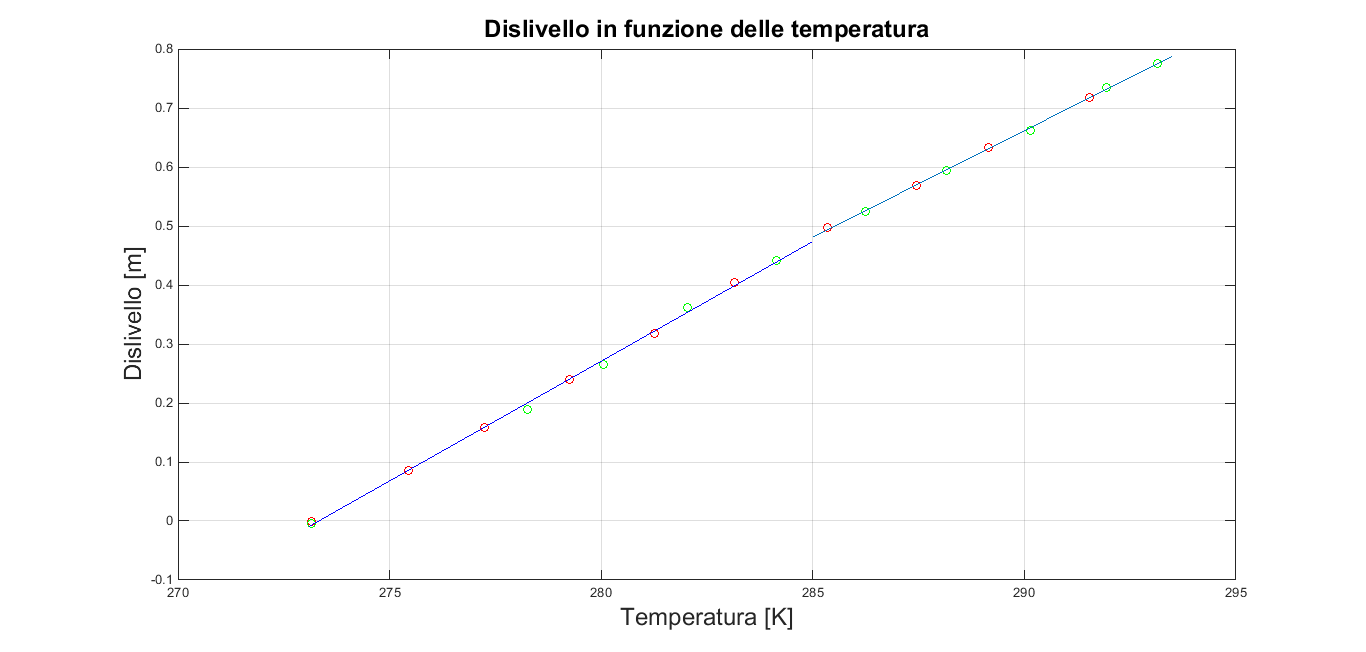
\includegraphics[width=\textwidth]{img/2}
\caption{Grafico di $\Delta h$ in funzione di $T$: 2 rette diverse per i dati divisi da 285 K}
\end{figure}

Iniziamo a valutare i dati al di sotto dei 285 K.\\
Procediamo nello stesso identico modo di prima e tramite regressione lineare troviamo la retta $h = A+B\theta$.
Otteniamo:
\[a =-11.0928 \pm 0.0289 \quad  b= 0.0406\pm 0.00010355\]
Il $\chi^2$ ci da: 231.5047. Decisamente troppo alto, molto probabilemente abbiamo sottostimato le incertezze sui valori, calcoliamo le incertezze a posteriori:
\begin{equation}
\label{eq:post}
\sigma(\Delta h)_{post} = \frac{1}{N-2}\sum_{i=1}^N(h-a-bT)^2
\end{equation}
Ci viene un incertezza a posteriori pari a $6.3\, mm$. È piuttosto difficile attriburla alla lettura del metro. In questa incertezza però innanzitutto contribuisce anche la risoluzione del termometro che non basta però a spiegare questa incertezza. Per comprenderne iL significato dobbiamo considerare la variazione di pressione atromosferica durante la sessione in cui si sono prese le misure. Questa analisi iniziale non ne tiene conto il suo effetto però si evidenzia bene in questa incertezza.\\
\newline
Studiamo ora l'andamento dei dati al di sopra dei 285K. Sempre allo stesso modo cerchiamo la retta $h = A+B\theta$ che interpreta meglio i nostri dati. Otteniamo:
\[a = -9.8096 \pm 0.0385 \quad  b= 0.0361 \pm 0.0001327\]
IL test del $\chi^2$ ci fornisce la bontà di questo fit: $\chi^2 = 48.5434$. Un po troppo alto rispetto a quello che volevamo. Procediamo dunque a calcolare l'incertezza a posteriori con l'equazione \eqref{eq:post} e otteniamo un incerteza a posteriori di $2.8\, mm$, che può essere comprensibile tenendo conto della risoluzioni di 1 millimetro del metro, della risoluzione del termometro trasferita e della variazione di pressione atmosferica durante l'acquisizione dei dati.


\subsection{Determinazione dello \emph{zero assoluto}}
Durante l'esperienza si è utilizzato un barometro in laboratorio per la misura della pressione atmosferica $P_A$ variabile nel tempo. Nel nostro manometro differenziale la pressione dovuta alla colonnina di acqua è data da: $\Delta P = \rho gh$. 
La pressione $P$ del nostro gas è quindi 
\begin{equation}
\label{eq:p}
P = P_A + \rho gh
\end{equation}
In appendice B è riportata la Tabella relativa alla pressione atmosferica misurata nel tempo, grazie a quella e all'equazione \eqref{eq:p} possiamo stimare la pressione $P$ del gas in funzione della temperatura.\\
Stima delle incertezze\\
\begin{table}[H]
	\centering
	\begin{tabular}{|c|c|} \hline
		\textbf{P {[Pa]} } & \textbf{T {[\degree C]} }  \\ \hline
		 &   \\ \hline
		 &   \\ \hline
		 &   \\ \hline
		 &   \\ \hline
		 &   \\ \hline
		 &   \\ \hline
		 &   \\ \hline
		 &   \\ \hline
		 &   \\ \hline
		 &   \\ \hline
		 &   \\ \hline
	\end{tabular}
	\caption{Pressione del gas $P$ in funzione della temperatura $T$}
\end{table}

Da inserire in grafico :)

Lo zero assoluto è rappresentato graficamente dall'intersezione tra la retta del dislivello $\Delta h$ in funzione della temperatura $T$ e l'asse delle ascisse.
Questo punto rappresenta la condizione $P = 0$.

\section{Analisi dati: secondo set}
\subsection{Pressione e temperatura}

\begin{table}[H]
\centering

	\begin{subtable}{.5\textwidth}
		\centering
		\begin{tabular}{|c|c|} \hline
			\textbf{$\Delta h {[cm]}$ } & \textbf{T {[\degree C]} }  \\ \hline
			-0.5 & 0  \\ \hline
			18.3 & 4.7  \\ \hline
			30.4 & 7.77  \\ \hline
			43.4 & 11.5  \\ \hline
			57.9 & 15.1  \\ \hline
			69 & 18.1  \\ \hline
			76.6 & 20  \\ \hline
		\end{tabular}
		\caption{Aumento della temperatura }
	\end{subtable}%
	\begin{subtable}{.5\textwidth}
	\centering
	\begin{tabular}{|c|c|} \hline
		\textbf{$\Delta h {[cm]}$ } & \textbf{T {[\degree C]} }  \\ \hline
		76.6 & 20  \\ \hline
		58.7 & 15  \\ \hline
		49.6 & 12.5  \\ \hline
		35 & 8.7  \\ \hline
		19.9 & 5.1  \\ \hline
		-0.2 & 0.16  \\ \hline
	\end{tabular}
	\caption{Diminuzione della temperatura }
\end{subtable}

\caption{Dislivello $\Delta h$ in funzione della temperatura $T$ }
\end{table}
In Tabella 3.a e Tabella 3.b troviamo riportati il secondo set di dati raccolti durante la nostra esperienza rispettivamente aumentando e diminuendo la temperatura del bagno termico.
Troviamo graficati tali dati in Figura 3. 


\section{Conclusioni: errori sistematici}
\subsection{Volume di gas non termalizzato con il bagno termico}
Una possibile causa di errore sistematico è la possibile presenza di gas non termalizzato con il bagno termico all'interno dell'ampolla.
È infatti possibile che il gas dell'ampolla presenti una parte di volume $V$ termalizzato con il bagno termico ed una parte di volume $v$ non termalizzato con il bagno termico e che si trova quindi a temperatura ambiente.
Considerando $n$ moli di gas nell'ampolla, l'equazione di stato diventa:
\begin{equation}
n R = P_0 \left[\frac{V}{T_0} + \frac{v}{T_a}\right] = P \left[\frac{V}{T} + \frac{v}{T_a}\right]
\end{equation}
dove $T_a$ rappresenta la temperatura ambiente.
Otteniamo quindi:
\begin{equation}
\frac{P_0 V}{T_0} \left[1 + v T_0 V T_a\right]= \frac{P V}{T} \left[1 + \frac{v T}{V T_a}\right]
\end{equation}
La relazione tra temperatura $T$  e pressione assoluta $P$ va quindi corretta, ottenendo quindi:
\begin{equation}
P = \left(\frac{P_0}{T_0}\right) \frac{1 + \left(\frac{v T_0}{V T_a} \right)}{1 + \left(\frac{v T}{V T_a}\right)} T = P_0 \frac{1 + \left(\frac {v T_0}{V T_a}\right)}{1 + \left(\frac{v T}{V T_a}\right)} \left(1 + \alpha T \right)
\end{equation}
Al crescere della temperatura quindi la pedenza della funzione $P(T)$ diminuisce.
Ad ogni modo, anche se il volume del gas dell'ampolla $v$ fosse effettivamente tutto termalizzato, nel caso reale andrebbe comunque applicata una correzione sulla pressione del tipo:
\begin{equation}
P_{mis} = \frac{n R T}{V + \frac{v T}{T_a}}
\end{equation}

\newpage
\begin{appendices}

\section{Metodo dei minimi quadrati}
Applicando il metodo dei minimi quadrati alla legge lineare $ y = A + Bx$ la discrepanza risulta:

\begin{equation}
\displaystyle\sum_{i=1}^{N}\frac{(y_i -A-Bx_i)^2}{(\sigma y_i)^2}
\end{equation}
\hspace{-1.8em}

Questa sommatoria è minimizzata da valori di A e B ottenuti come:

\begin{equation}
\label{eq:a}
A = \frac{(\sum_i w_i x_i^2)(\sum_i w_i y_i)-(\sum_i w_i x_i)(\sum_i w_i x_i y_i)}{\Delta} 
\end{equation}
e
\begin{equation}
\label{eq:b}
B = \frac{(\sum_i w_i)(\sum_i w_i y_i x_i)-(\sum_i w_i y_i)(\sum_i w_i x_i)}{\Delta}
\end{equation}
Dove abbiamo:
\[ \Delta = (\sum_i w_i)(\sum_i w_i x_i^2)-(\sum_i w_i x_i)^2  \quad \quad  w_i = \frac{1}{(\sigma y_i)^2}\]
\hspace{-1.8em}
Le incertezze sui parametri sono date da:

\begin{equation} 
\label{eq:sasb}
(\sigma A)^2 = \frac{\sum_i w_i x_i^2}{\Delta}\quad \quad (\sigma B)^2 = \frac{\sum_i w_i}{\Delta}
\end{equation}

\section{Pressione atmosferica}

\begin{table}[H]
	\centering
	\begin{tabular}{|c|c|} \hline
		\textbf{P {[pa]} } & \textbf{ORA {[hh:mm]} }  \\ \hline
		130.5 & 2.306  \\ \hline
		130.5 & 2.306  \\ \hline
		130.5 & 2.306  \\ \hline
		130.5 & 2.306  \\ \hline
	\end{tabular}
	\caption{Pressione del gas in funzione della temperatura}
\end{table}


\end{appendices}



\end{document}
